\documentclass[10pt]{beamer}
\usepackage[utf8]{inputenc}
\usepackage[french]{babel}
\usepackage[T1]{fontenc}
\usefonttheme{serif} 
\usepackage[document]{ragged2e}
\usetheme{Warsaw}

\defbeamertemplate*{footline}{shadow theme}
{%
  \leavevmode%
  \hbox{\begin{beamercolorbox}[wd=.5\paperwidth,ht=2.5ex,dp=1.125ex,leftskip=.3cm plus1fil,rightskip=.3cm]{author in head/foot}%
    \usebeamerfont{author in head/foot}\insertframenumber\,/\,\inserttotalframenumber\hfill\insertshortauthor
  \end{beamercolorbox}%
  \begin{beamercolorbox}[wd=.5\paperwidth,ht=2.5ex,dp=1.125ex,leftskip=.3cm,rightskip=.3cm plus1fil]{title in head/foot}%
    \usebeamerfont{title in head/foot}\insertshorttitle%
  \end{beamercolorbox}}%
  \vskip0pt%
}

\makeatletter
\newcommand\titlegraphicii[1]{\def\inserttitlegraphicii{#1}}
\titlegraphicii{}
\setbeamertemplate{title page}
{
  \vbox{}
   {\usebeamercolor[fg]{titlegraphic}\inserttitlegraphic\hfill\inserttitlegraphicii\par}
  \begin{centering}
    \begin{beamercolorbox}[sep=8pt,center]{institute}
      \usebeamerfont{institute}\insertinstitute
    \end{beamercolorbox}
    \begin{beamercolorbox}[sep=8pt,center]{title}
      \usebeamerfont{title}\inserttitle\par%
      \ifx\insertsubtitle\@empty%
      \else%
        \vskip0.25em%
        {\usebeamerfont{subtitle}\usebeamercolor[fg]{subtitle}\insertsubtitle\par}%
      \fi%     
    \end{beamercolorbox}%
    \vskip1em\par
    \begin{beamercolorbox}[sep=8pt,center]{date}
      \usebeamerfont{date}\insertdate
    \end{beamercolorbox}%\vskip0.5em
    \begin{beamercolorbox}[sep=8pt,center]{author}
      \usebeamerfont{author}\insertauthor
    \end{beamercolorbox}
  \end{centering}
  %\vfill
}


\makeatother
%\author{Rosetta Lab}
\title{Projet Sudoku – ESP Dakar 2019}
\institute{Ecole Supérieure Polytechnique de Dakar \\ Département Génie Informatique}
\date{02 Mars 2019}
\titlegraphic{
\includegraphics[height=1.5cm,width=2cm]{ESP.jpg}}
\titlegraphicii{
\includegraphics[height=1.5cm,width=2cm]{UCAD.png}}

\begin{document}
\small
\begin{frame}[plain]
\maketitle
\begin{tabular}[t]{@{}l@{\hspace{3pt}}p{.33\textwidth}@{}}
\underline{Participants :} & Arfang FAYE \\
& Fassou Mathias Niamy 


\end{tabular}%
\footnotesize
\begin{tabular}[t]{@{}l@{\hspace{3pt}}p{.3\textwidth}@{}}
\underline{Professeur :} & M. Alain FAYE 
\end{tabular}%
\end{frame}

{
\renewcommand{\insertnavigation}[1]{}
\setbeamertemplate{headline}{}

\begin{frame}
\begin{center}
\end{center}
\begin{center}
\underline{\textbf{PLAN}}
\end{center}

\tableofcontents
\end{frame}
}


\begin{frame}
\section{Objectif}
\begin{block}{Objectif}
L'objectif de ce projet est de modéliser le jeu du Sudoku par un programme mathématique, le coder et le tester sur le
solveur glpk (licence gnu).
\end{block}
\end{frame}


\begin{frame}
\section{Les contraintes}
\small
Soit $i$, $j$, $k$ des indices comprisent entre 1 et 9 utilisé comme suit :\\
$i$ représente l'indice de la ligne courante \\
$j$ représente l'indice de la colonne courante \\
$k$ représente l'indice du sous-carré courante (3x3) \\
\begin{enumerate}
\item[1)] Soit $X_{i,j,k}$ définie comme suit :
\begin{equation}
X_{i,j,k} =
\begin{cases}
1 & \text{si la valeur $k$ est affectée à la case $i$,$j$ est  } 
\\
0 & \text{sinon } 
\end{cases}
\end{equation}
\item[2)]Pour chaque valeur fixée par la matrice de départ : $X_{i,j,k} = 1$
\item[3)]Chaque case ne doit contenir qu'une et une seule valeur : $$\sum_{k=1}^{9} X_{i,j,k} = 1$$
\item[4)]Chaque valeur doit être unique sur la ligne : $$\sum_{i=1}^{9} X_{i,j,k} = 1$$
\end{enumerate}
\end{frame}

\begin{frame}
\begin{enumerate}
\item[5)]chaque valeur doit être unique sur la colonne : $$\sum_{j=1}^{9} X_{i,j,k} = 1$$
\item[6)] Chaque valeur doit être présent une et une seul fois dans chacun des sous-carrés : \\
$$\mathop{\sum_{j=3p-2}^{3p}\sum_{i=3p-2}^{3q}} X_{i,j,k} = 1$$ avec $p$, $q$ = 1 à 3
\end{enumerate}
Dans le cadre de cette résolution nous avons pas besoin de but (équation à maximiser ou minimiser)
\end{frame}

\begin{frame}[fragile]
\section{Visualisation des resultats}
Le resultat de la résolution donne une matrice de ce type : \\
\begin{center}
\begin{tiny}
\begin{verbatim}
[[1,1,8],[1,2,9],[1,3,3],[1,4,5],[1,5,1],[1,6,6],[1,7,7],[1,8,4],[1,9,2],
[2,1,7],[2,2,1],[2,3,4],[2,4,8],[2,5,2],[2,6,9],[2,7,5],[2,8,6],[2,9,3],
[3,1,2],[3,2,6],[3,3,5],[3,4,3],[3,5,4],[3,6,7],[3,7,1],[3,8,9],[3,9,8],
[4,1,4],[4,2,5],[4,3,1],[4,4,7],[4,5,3],[4,6,2],[4,7,6],[4,8,8],[4,9,9],
[5,1,9],[5,2,2],[5,3,8],[5,4,6],[5,5,5],[5,6,1],[5,7,3],[5,8,7],[5,9,4],
[6,1,6],[6,2,3],[6,3,7],[6,4,9],[6,5,8],[6,6,4],[6,7,2],[6,8,5],[6,9,1],
[7,1,3],[7,2,8],[7,3,9],[7,4,2],[7,5,6],[7,6,5],[7,7,4],[7,8,1],[7,9,7],
[8,1,5],[8,2,4],[8,3,2],[8,4,1],[8,5,7],[8,6,8],[8,7,9],[8,8,3],[8,9,6],
[9,1,1],[9,2,7],[9,3,6],[9,4,4],[9,5,9],[9,6,3],[9,7,8],[9,8,2],[9,9,5]]
\end{verbatim}
\end{tiny}
\end{center}

en utilisant le visualisateur de solution nous obtenons la figure suivante :
\begin{center}
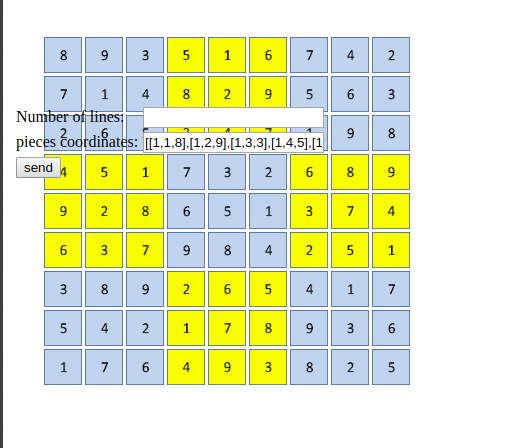
\includegraphics[scale=0.3]{sudoku_diabolique_resultats.png}
\end{center}
\end{frame}

\end{document}